\documentclass{article}

% 导入中文宏包
\usepackage{array}
\usepackage{caption}
\usepackage{ctex}
\usepackage{hyperref}
% 设置页面边距
\usepackage{geometry}
\usepackage{graphicx}
\geometry{a4paper, left=2cm, right=2cm, top=3cm, bottom=4cm}

% 设置标题、作者和日期
\title{Python入门与视觉应用}
\author{23020007073  刘畅}

\begin{document}

% 生成标题、作者和日期
\maketitle

% 心得报告正文
\section{实验目的}
掌握Python的基本编程方法,能够编写简单的程序。

了解图像处理的基本概念,能够通过Python进行图像读取、显示和保存。

\section{练习内容}

\subsection{命令行学习5个例子}
1.创建文件夹:
\begin{verbatim}
	mkdir new_folder
\end{verbatim}
\noindent
\begin{minipage}{\linewidth}
	\centering
	% 插入图片
	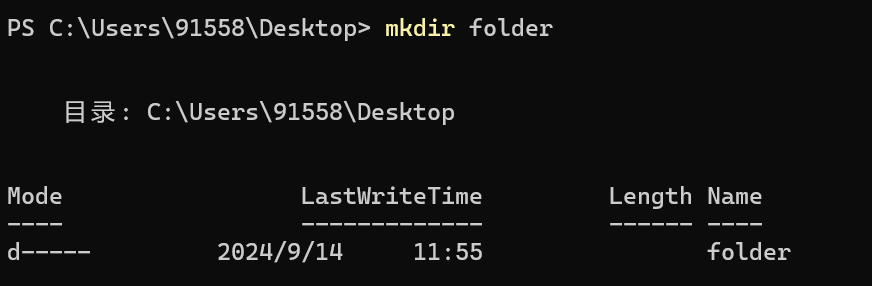
\includegraphics[width=0.5\linewidth]{mkdir.png}
	% 图片标题
	\captionof{figure}{创建文件夹}
	\label{fig:example}
\end{minipage}


2.删除文件夹:
\begin{verbatim}
	rmdir /s /q folder_name
\end{verbatim}


\noindent
\begin{minipage}{\linewidth}
	\centering
	% 插入图片
	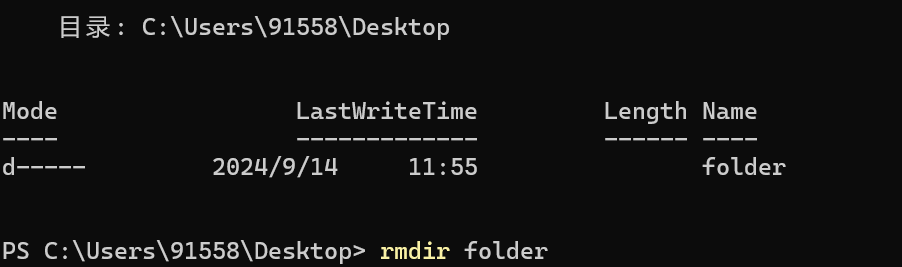
\includegraphics[width=0.5\linewidth]{rmdir.png}
	% 图片标题
	\captionof{figure}{删除文件夹}
	\label{fig:example}
\end{minipage}


3.文本文件的创立与写入
\begin{verbatim}
	echo "Hello, World!" > hello.txt
\end{verbatim}


\noindent
\begin{minipage}{\linewidth}
	\centering
	% 插入图片
	
\includegraphics[width=0.5\linewidth]{echo.png}
	% 图片标题
	\captionof{figure}{文本文件的创立与写入}
	\label{fig:example}
\end{minipage}


4.type example.txt
查看文件内容

\noindent
\begin{minipage}{\linewidth}
	\centering
	% 插入图片
	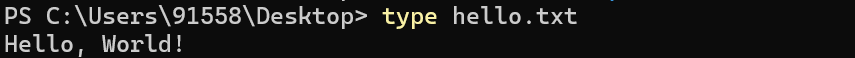
\includegraphics[width=0.5\linewidth]{type.png}
	% 图片标题
	\captionof{figure}{列表的输出结果}
	\label{fig:example}
\end{minipage}

5.wmic memorychip list brief
查看内存信息

\noindent
\begin{minipage}{\linewidth}
	\centering
	% 插入图片
	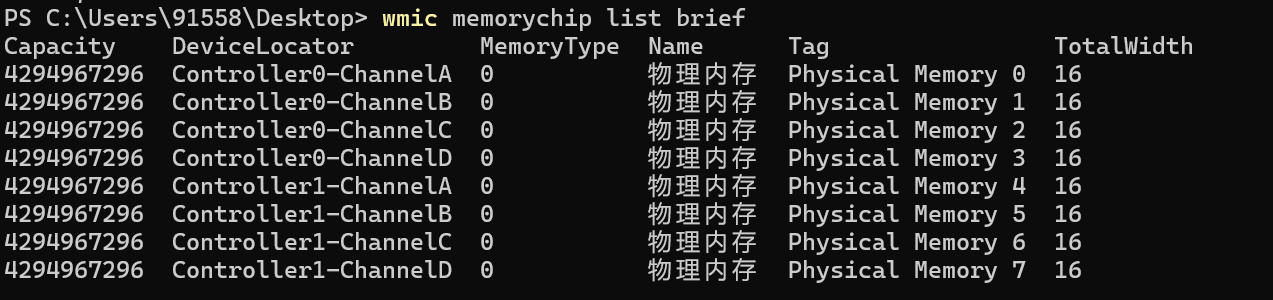
\includegraphics[width=0.5\linewidth]{wmic.png}
	% 图片标题
	\captionof{figure}{内存信息}
	\label{fig:example}
\end{minipage}

\subsection{Python样例10个}

1.print()打印的意思
print("hello,world")

\noindent
\begin{minipage}{\linewidth}
  \centering
  % 插入图片
  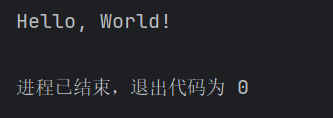
\includegraphics[width=0.5\linewidth]{print.png}
  % 图片标题
  \captionof{figure}{用print来打印内容}
  \label{fig:example}
\end{minipage}


2.条件语句的使用
\begin{verbatim}
    x=1 y=8
    if x > y:
      print("x is bigger than y")
    else:
      print("x is not bigger than y")

 \end{verbatim}


\noindent
\begin{minipage}{\linewidth}
  \centering
  % 插入图片
  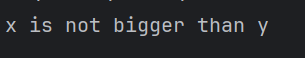
\includegraphics[width=0.5\linewidth]{if.png}
  % 图片标题
  \captionof{figure}{条件语句输出结果}
  \label{fig:example}
\end{minipage}

3.循环语句的使用
 \begin{verbatim}
     for i in [1, 2, 3, 4, 5]:
        print(i)
 \end{verbatim}

\noindent
\begin{minipage}{\linewidth}
  \centering
  % 插入图片
  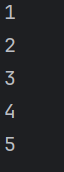
\includegraphics[width=0.5\linewidth,height=6cm]{for.png}
  % 图片标题
  \captionof{figure}{循环语句的使用}
  \label{fig:example}
\end{minipage}

4.函数的定义与使用
\begin{verbatim}
      def greet():
        print("Hello, Python") 
      greet()
\end{verbatim}

\noindent
\begin{minipage}{\linewidth}
 \centering
  % 插入图片
  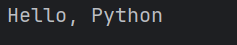
\includegraphics[width=0.5\linewidth]{def.png}
  % 图片标题
  \captionof{figure}{函数的定义与使用}
  \label{fig:example}
\end{minipage}



5.列表的使用
\begin{verbatim}
    list = [1, 2, 3, 4, 5]
    print(list[0])
\end{verbatim}


\noindent
\begin{minipage}{\linewidth}
 \centering
  % 插入图片
  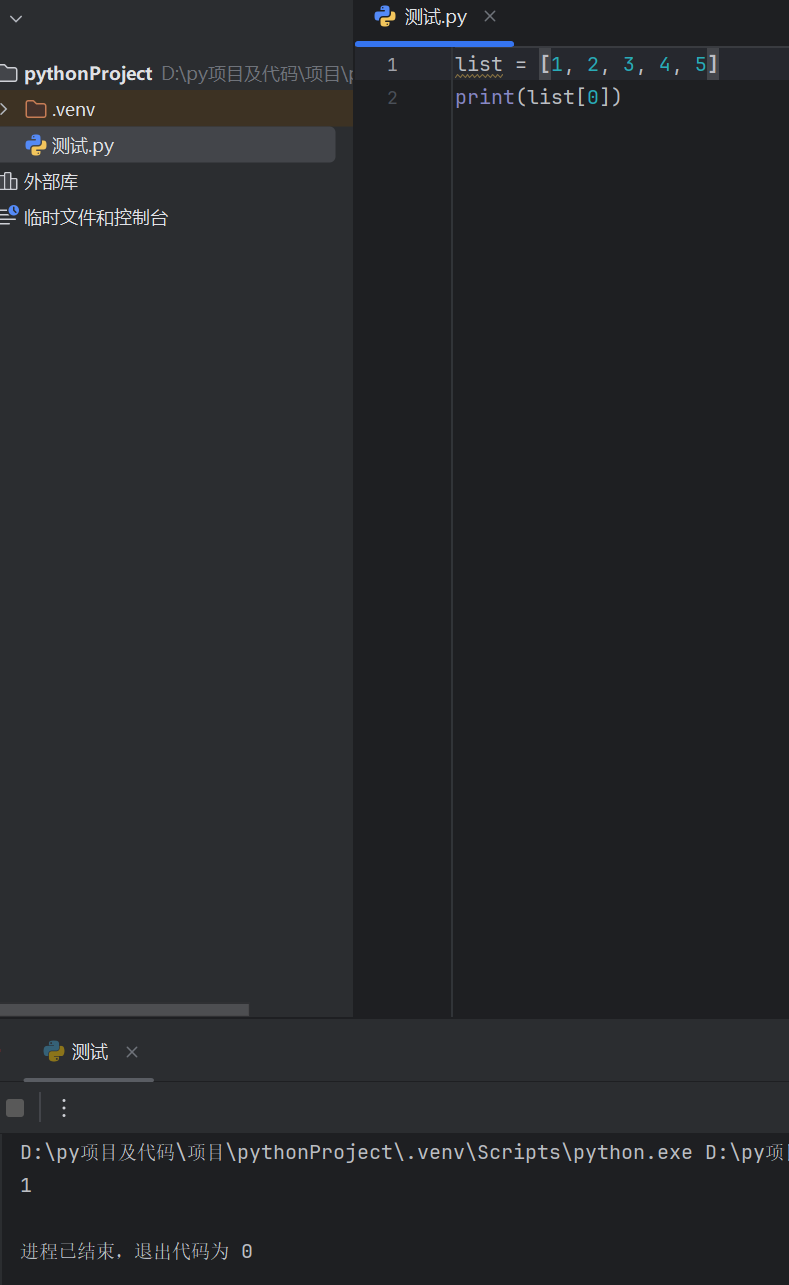
\includegraphics[width=0.5\linewidth]{list.png}
  % 图片标题
  \captionof{figure}{列表的输出结果}
  \label{fig:example}
\end{minipage}

6.字典的使用:
\begin{verbatim}
    person = {
        '名字': '李华',
        '年龄': 20,
        '城市': '青岛',
        '职业': '学生'
    }
    
    # 访问字典中的数据
    print(person['名字'])  
    print(person['职业'])
\end{verbatim}



\noindent
\begin{minipage}{\linewidth}
 \centering
  % 插入图片
  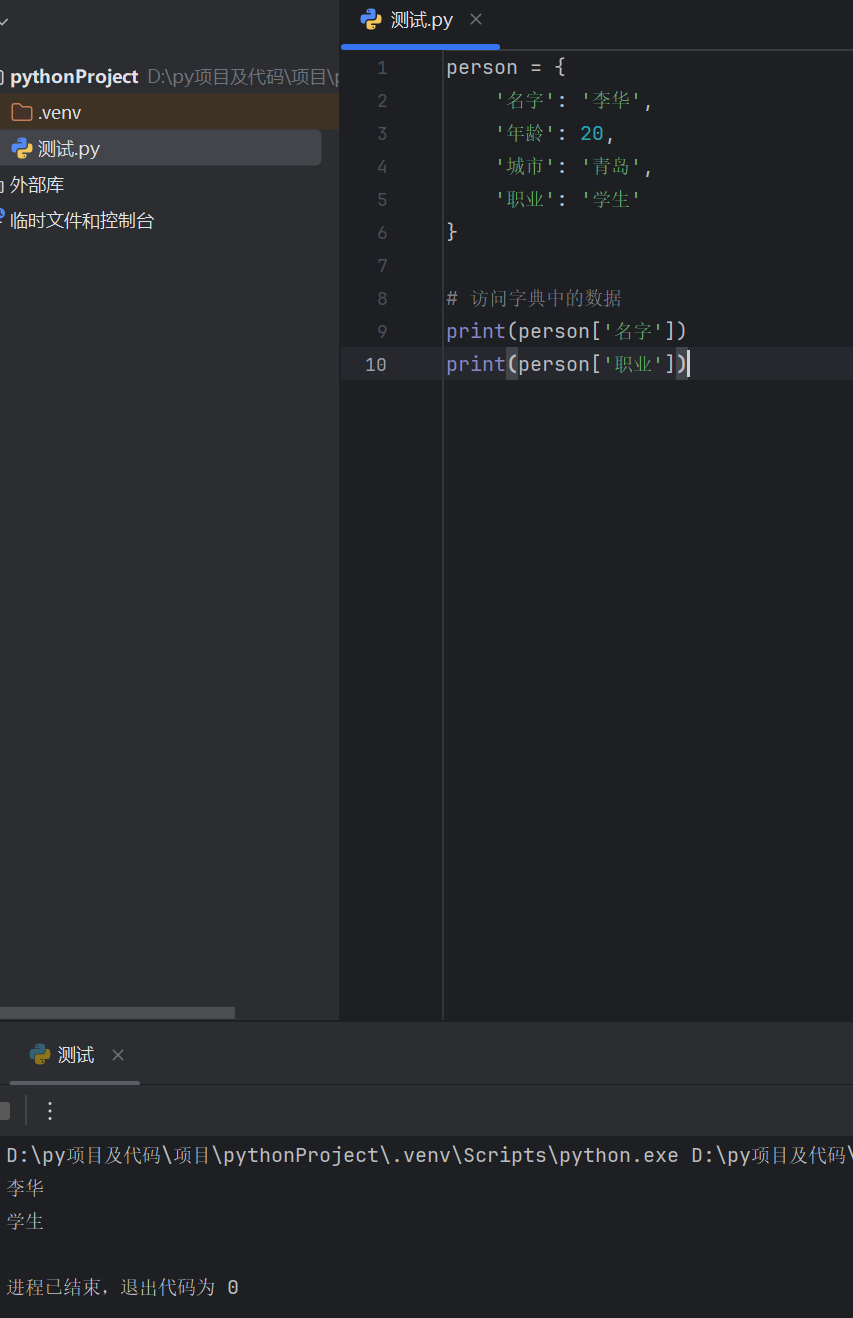
\includegraphics[width=0.5\linewidth]{zidian.png}
  % 图片标题
  \captionof{figure}{字典的输出结果}
  \label{fig:example}
\end{minipage}

7.元组的使用:
\begin{verbatim}
    yuanzu= (123, "work", 258)
    print(yuanzu[1])
\end{verbatim}


\noindent
\begin{minipage}{\linewidth}
 \centering
  % 插入图片
  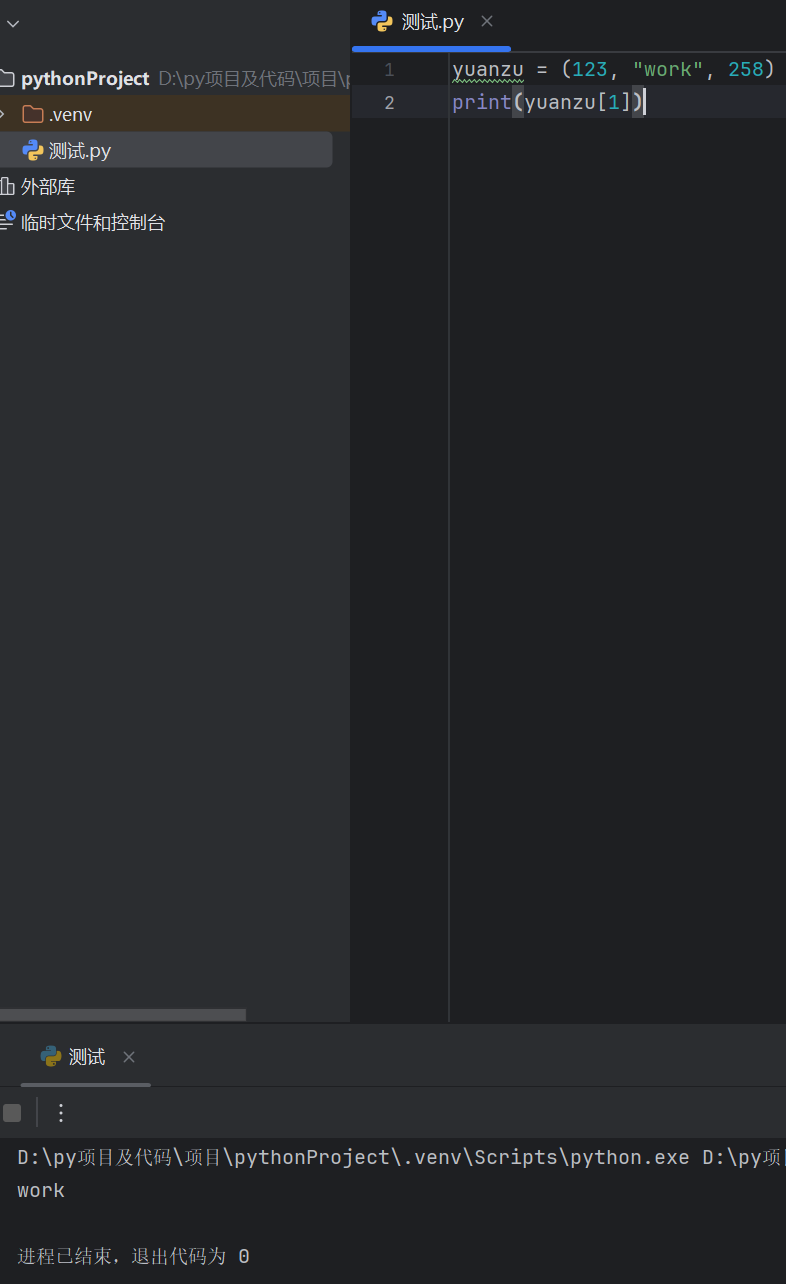
\includegraphics[width=0.5\linewidth]{yuanzu.png}
  % 图片标题
  \captionof{figure}{元组的输出结果}
  \label{fig:example}
\end{minipage}


8.程序和用户的交互:
\begin{verbatim}
    number = int(input("请输入一个整数:"))
    print("您输入的整数是:", number)
\end{verbatim}

\noindent
\begin{minipage}{\linewidth}
 \centering
  % 插入图片
  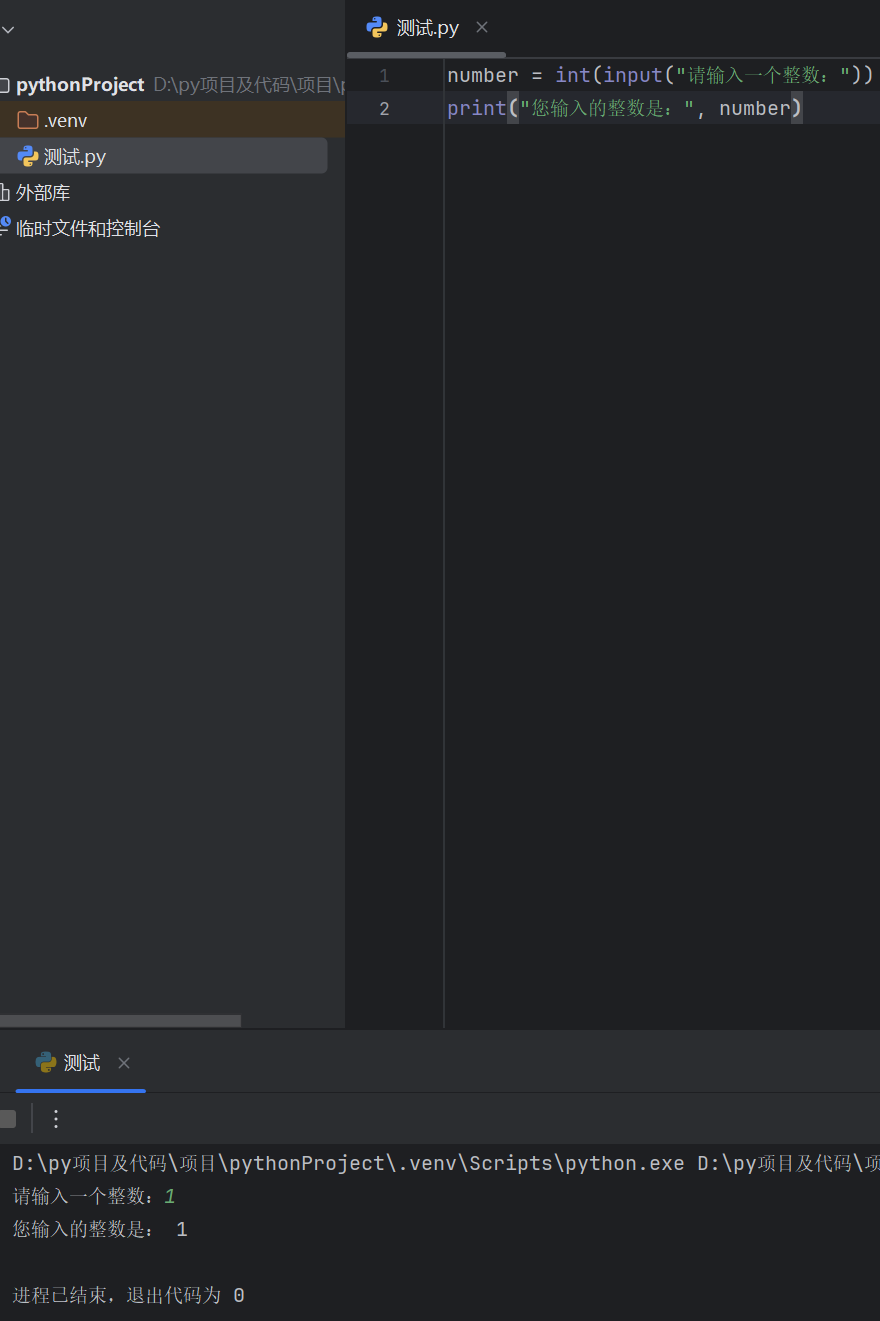
\includegraphics[width=0.5\linewidth]{jiaohu.png}
  % 图片标题
  \captionof{figure}{程序和用户的交互}
  \label{fig:example}
\end{minipage}



9. 类的使用:
\begin{verbatim}
class Class:
	def __init__(self, chinese, math, english):
		self.chinese = chinese
		self.math = math
		self.english = english

	def describe_class(self):
		return f"{self.chinese} {self.math} {self.english}"
myclass = Class('Yuwen', 'Shuxue', 'Yingyu')

print(myclass.describe_class())
\end{verbatim}

\begin{minipage}{\linewidth}
    \centering
     % 插入图片
     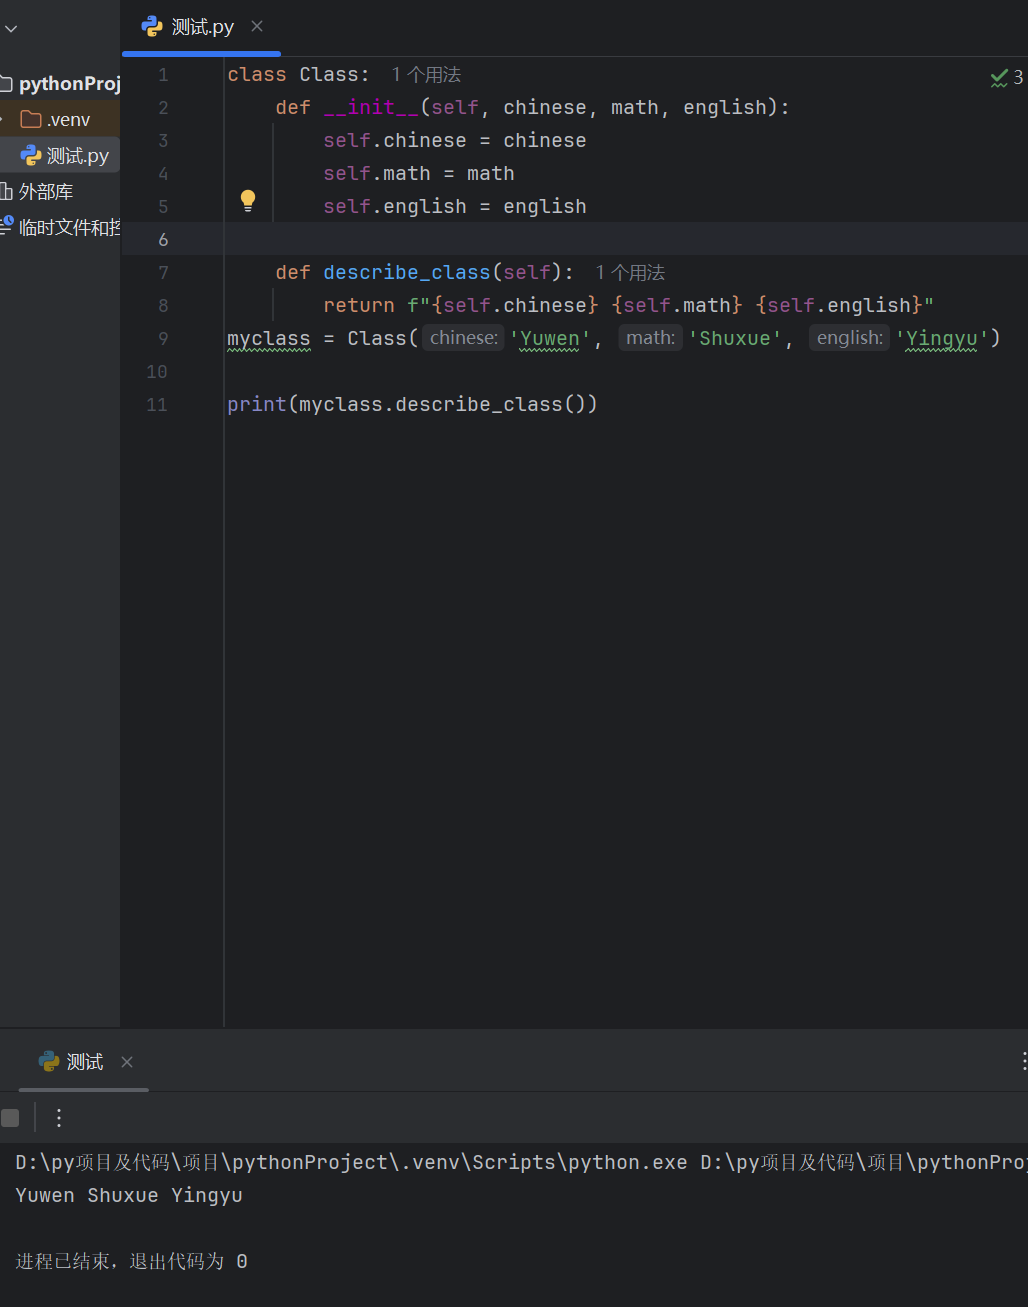
\includegraphics[width=0.5\linewidth]{class.png}
     % 图片标题
     \captionof{figure}{类的使用}
     \label{fig:example}
\end{minipage}


10.文件的写入和读取
\begin{verbatim}
    with open('example.txt', 'w') as file:
       file.write('Hello, World!')
    with open('example.txt', 'r') as file:
       content = file.read()
    print(content)
\end{verbatim}


\noindent
\begin{minipage}{\linewidth}
 \centering
  % 插入图片
  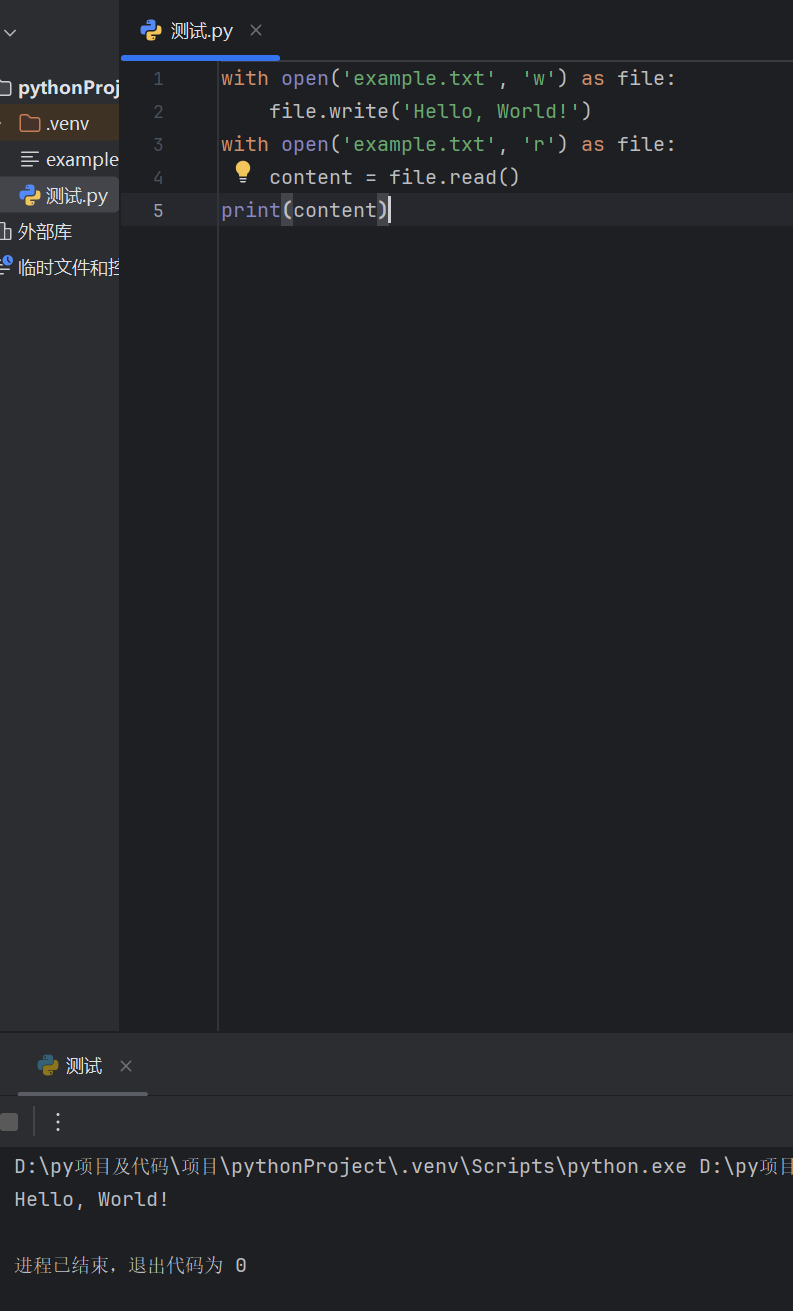
\includegraphics[width=0.5\linewidth]{file.png}
  % 图片标题
  \captionof{figure}{文件的写入和读取}
  \label{fig:example}
\end{minipage}



\subsection{Python视觉应用样例5个}
1.图像灰度变换
  \begin{verbatim}
     from PIL import Image
      # 读取图像
     image = Image.open('ceshi.jpg') 
      # 显示图像
     image.show()
      # 转换为灰度图像
     gray_image = image.convert('L')
     gray_image.show()
  \end{verbatim}

\noindent
\begin{minipage}{\linewidth}
 \centering
  % 插入图片
  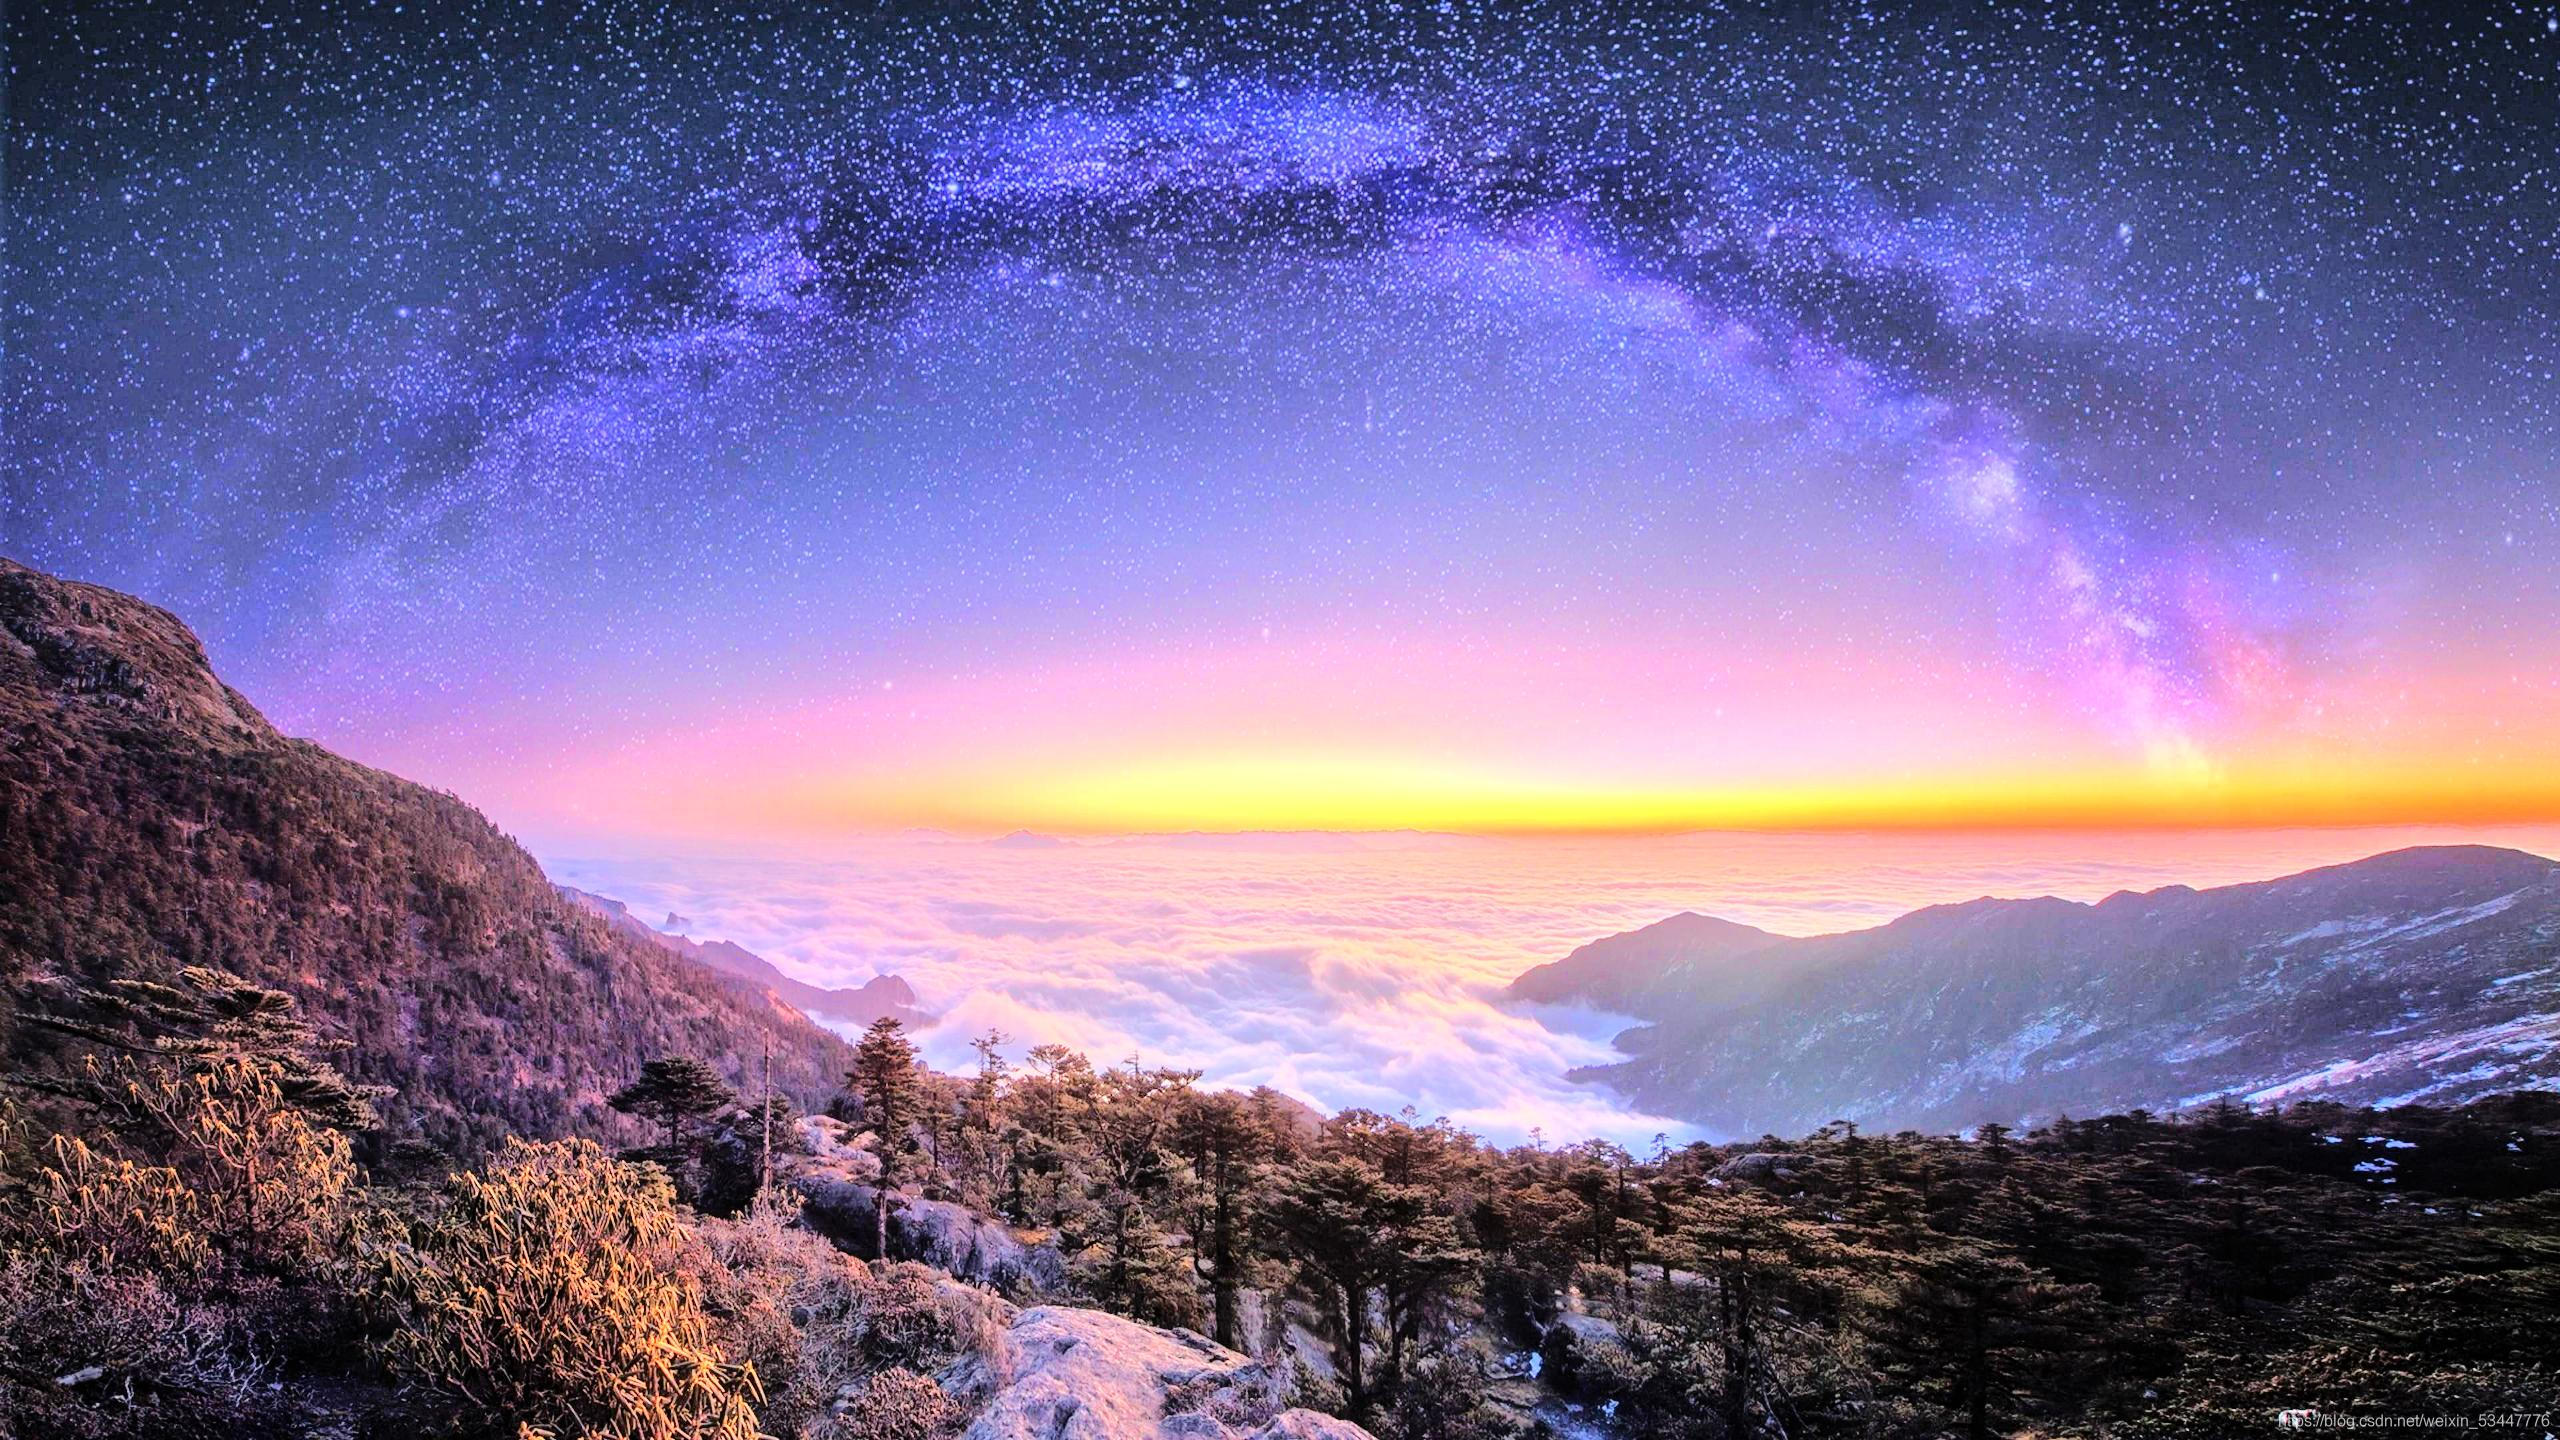
\includegraphics[width=0.5\linewidth]{ceshi.jpg}
  % 图片标题
  \captionof{figure}{灰度变换前}
  \label{fig:example}
\end{minipage}

\noindent
\begin{minipage}{\linewidth}
 \centering
  % 插入图片
  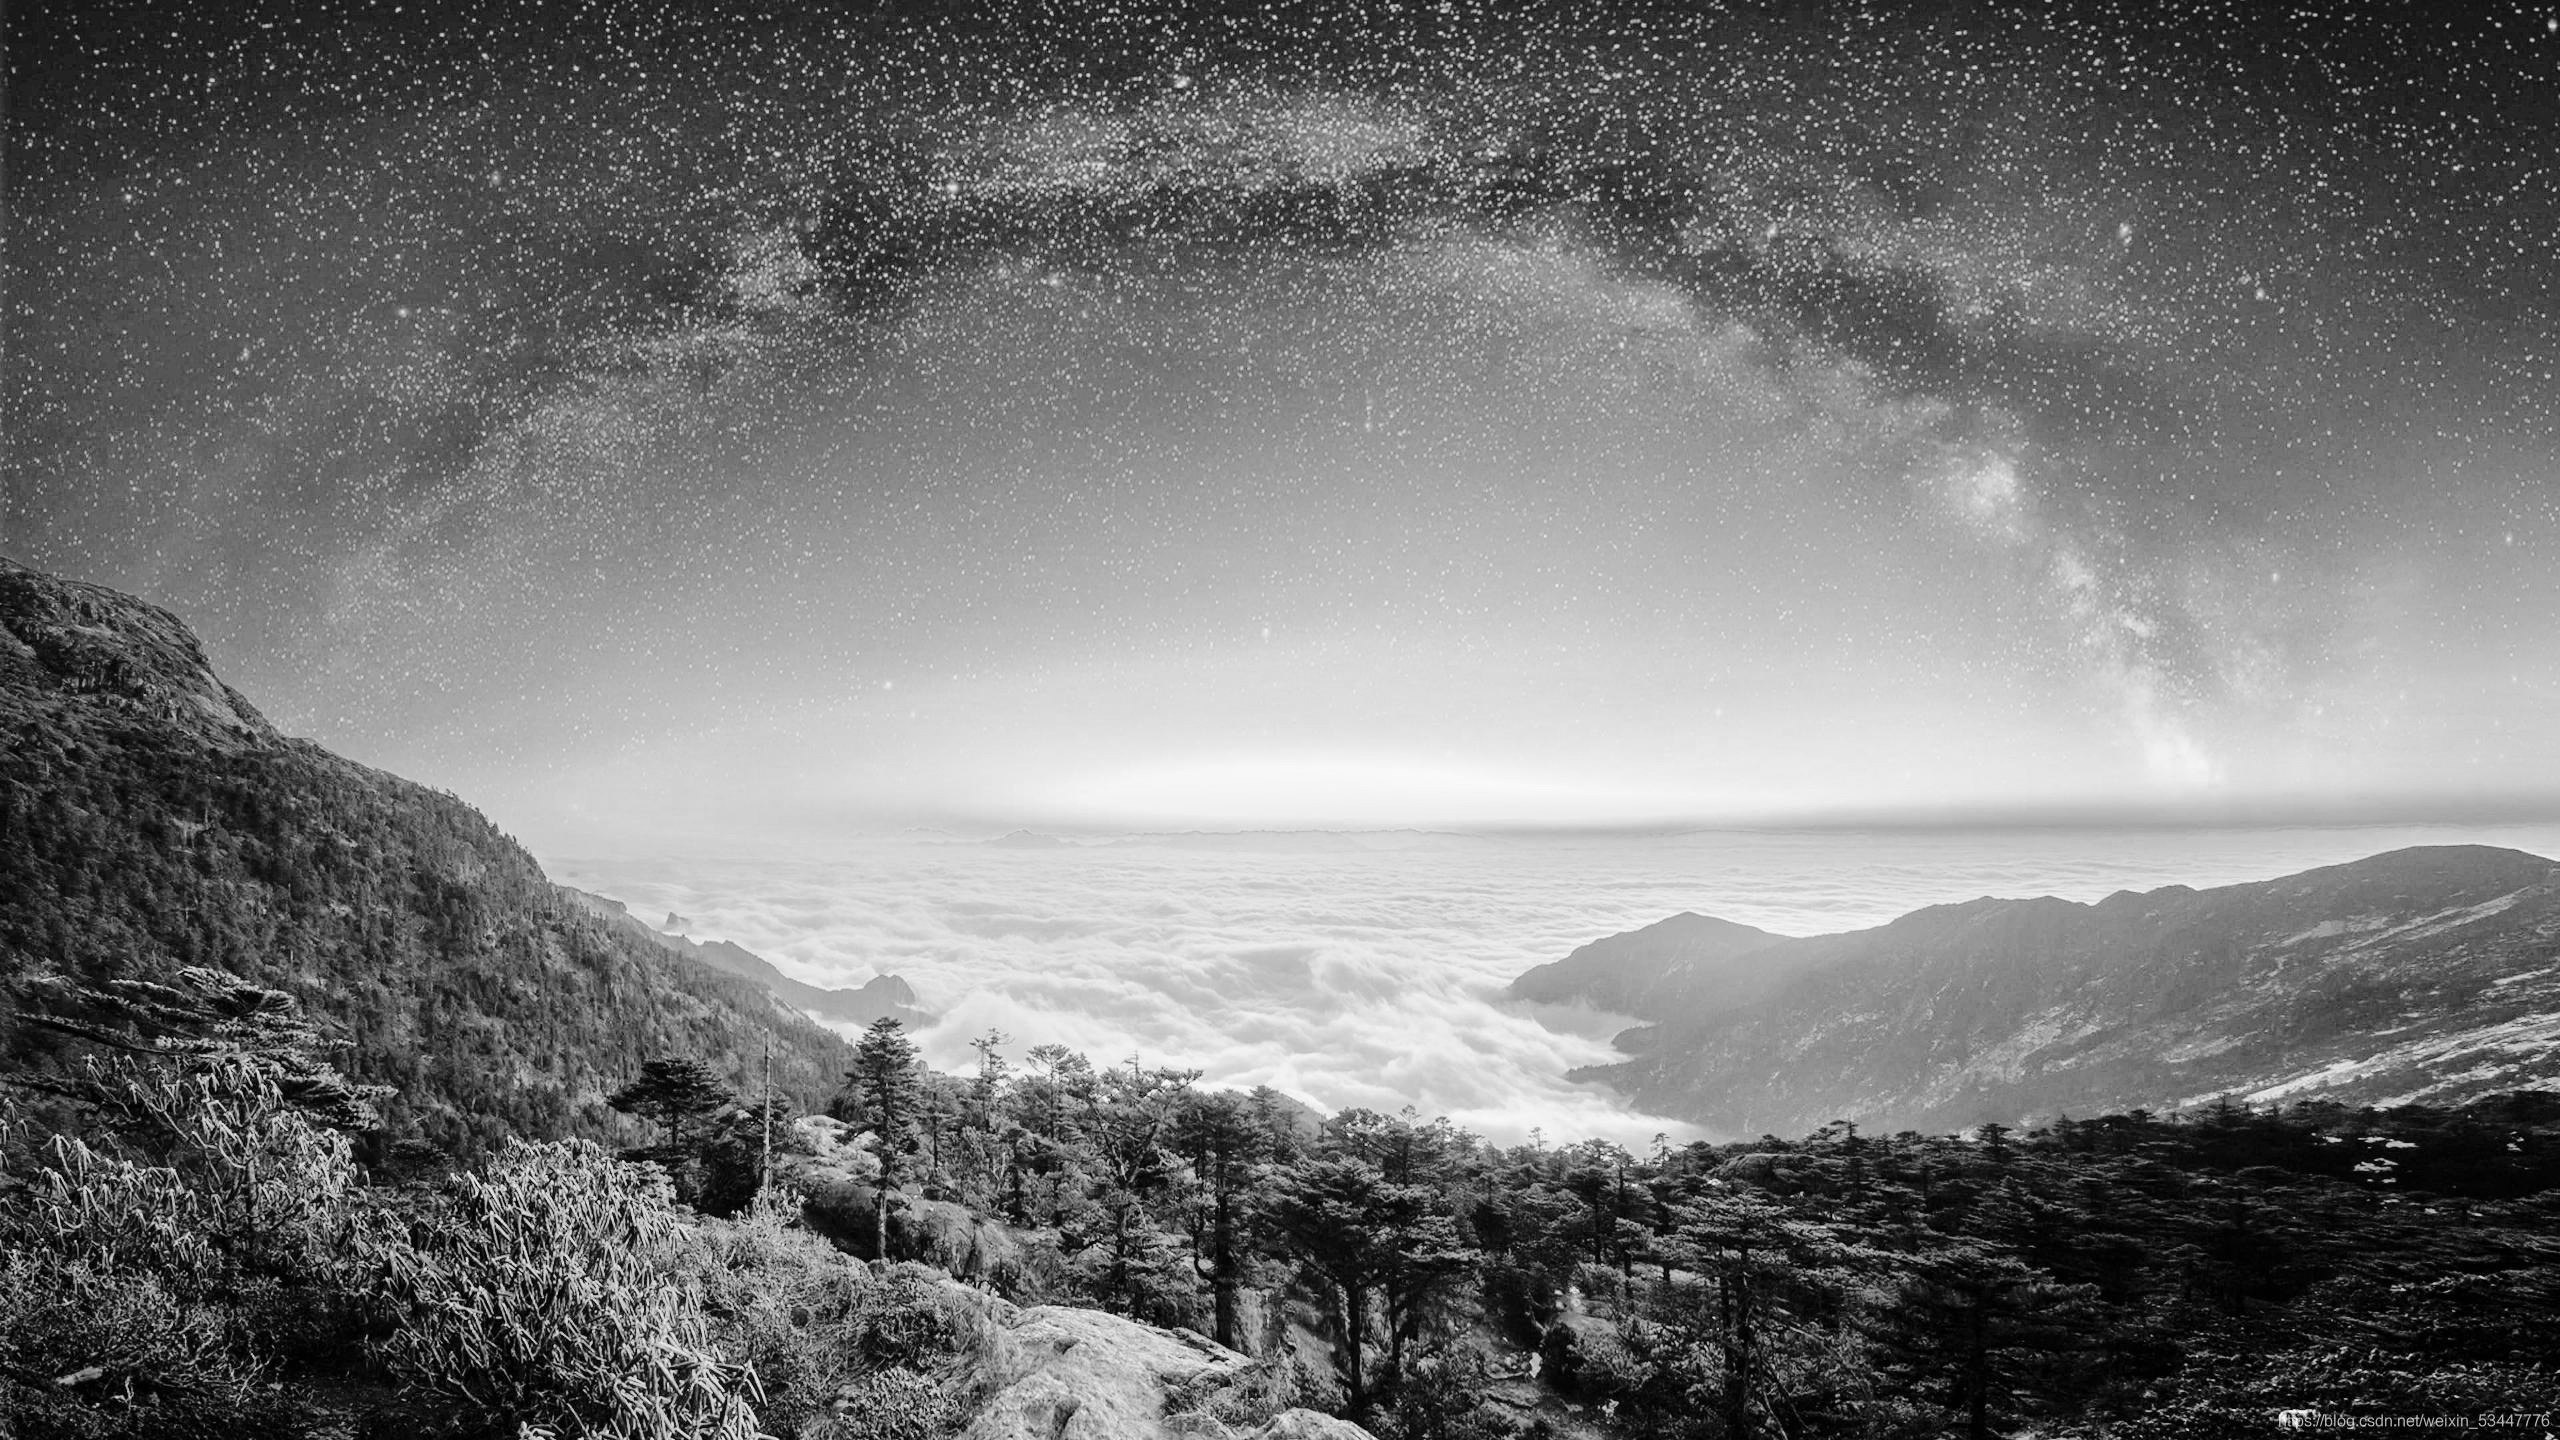
\includegraphics[width=0.5\linewidth]{huise.png}
  % 图片标题
  \captionof{figure}{灰度变换后}
  \label{fig:example}
\end{minipage}

2.利用Matplotlib完成折线图的绘制
    \begin{verbatim}
      import matplotlib.pyplot as plt
      import numpy as np
      x = np.linspace(0, 10, 100)  # 生成从0到10的100个点
      y = np.sin(x) + np.random.normal(0, 0.1, 100)  # 生成正弦曲线并添加一些随机噪声
      # 创建图形和轴
      plt.figure(figsize=(10, 6))  # 设置图形的大小
      plt.plot(x, y, label='sin(x) + noise', color='blue')  # 绘制折线图
      # 添加标题和标签
      plt.title('Simple Plot')
      plt.xlabel('X axis')
      plt.ylabel('Y axis')
      # 添加图例
      plt.legend()
      # 显示网格(可选)
      plt.grid(True)
      # 显示图形
      plt.show()
   \end{verbatim}


\noindent
\begin{minipage}{\linewidth}
 \centering
  % 插入图片
  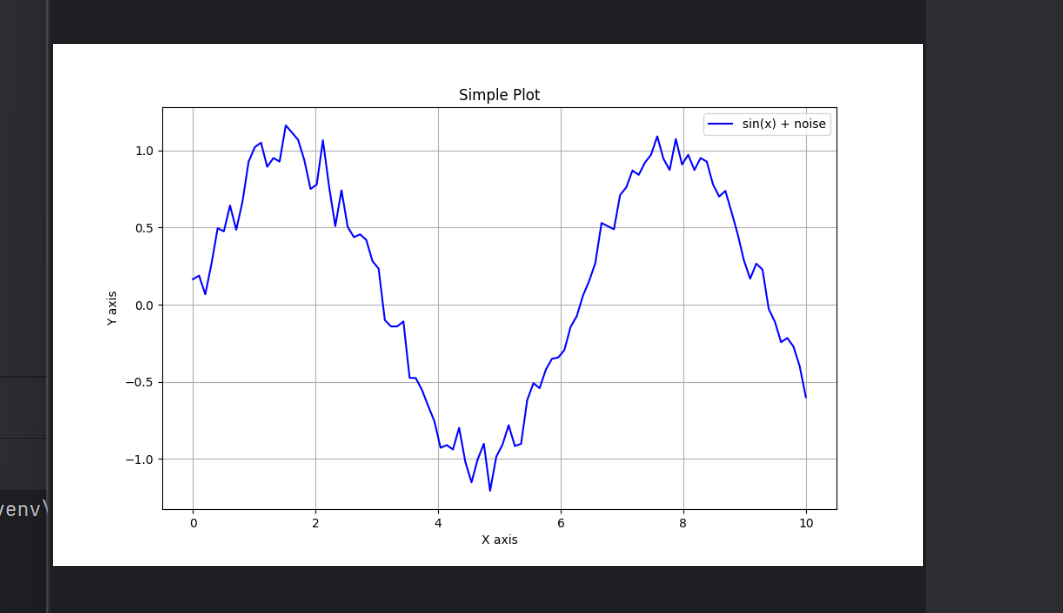
\includegraphics[width=0.5\linewidth]{xian.png}
  % 图片标题
  \captionof{figure}{绘制的折线图}
  \label{fig:example}
\end{minipage}

3.图像模糊
   \begin{verbatim}
      from PIL import Image
      import numpy as np
      import cv2
      # 读取图像
      image = Image.open('ceshi.jpg')
      # 转换图像为numpy数组
      image_np = np.array(image)
      # 应用均值模糊
      blurred_image_np = cv2.blur(image_np, (15, 15))
      # 转换numpy数组回PIL图像
      blurred_image = Image.fromarray(blurred_image_np)
      # 显示原始图像和均值模糊后的图像
      image.show()
      blurred_image.show()
  \end{verbatim}

\noindent
\begin{minipage}{\linewidth}
 \centering
  % 插入图片
  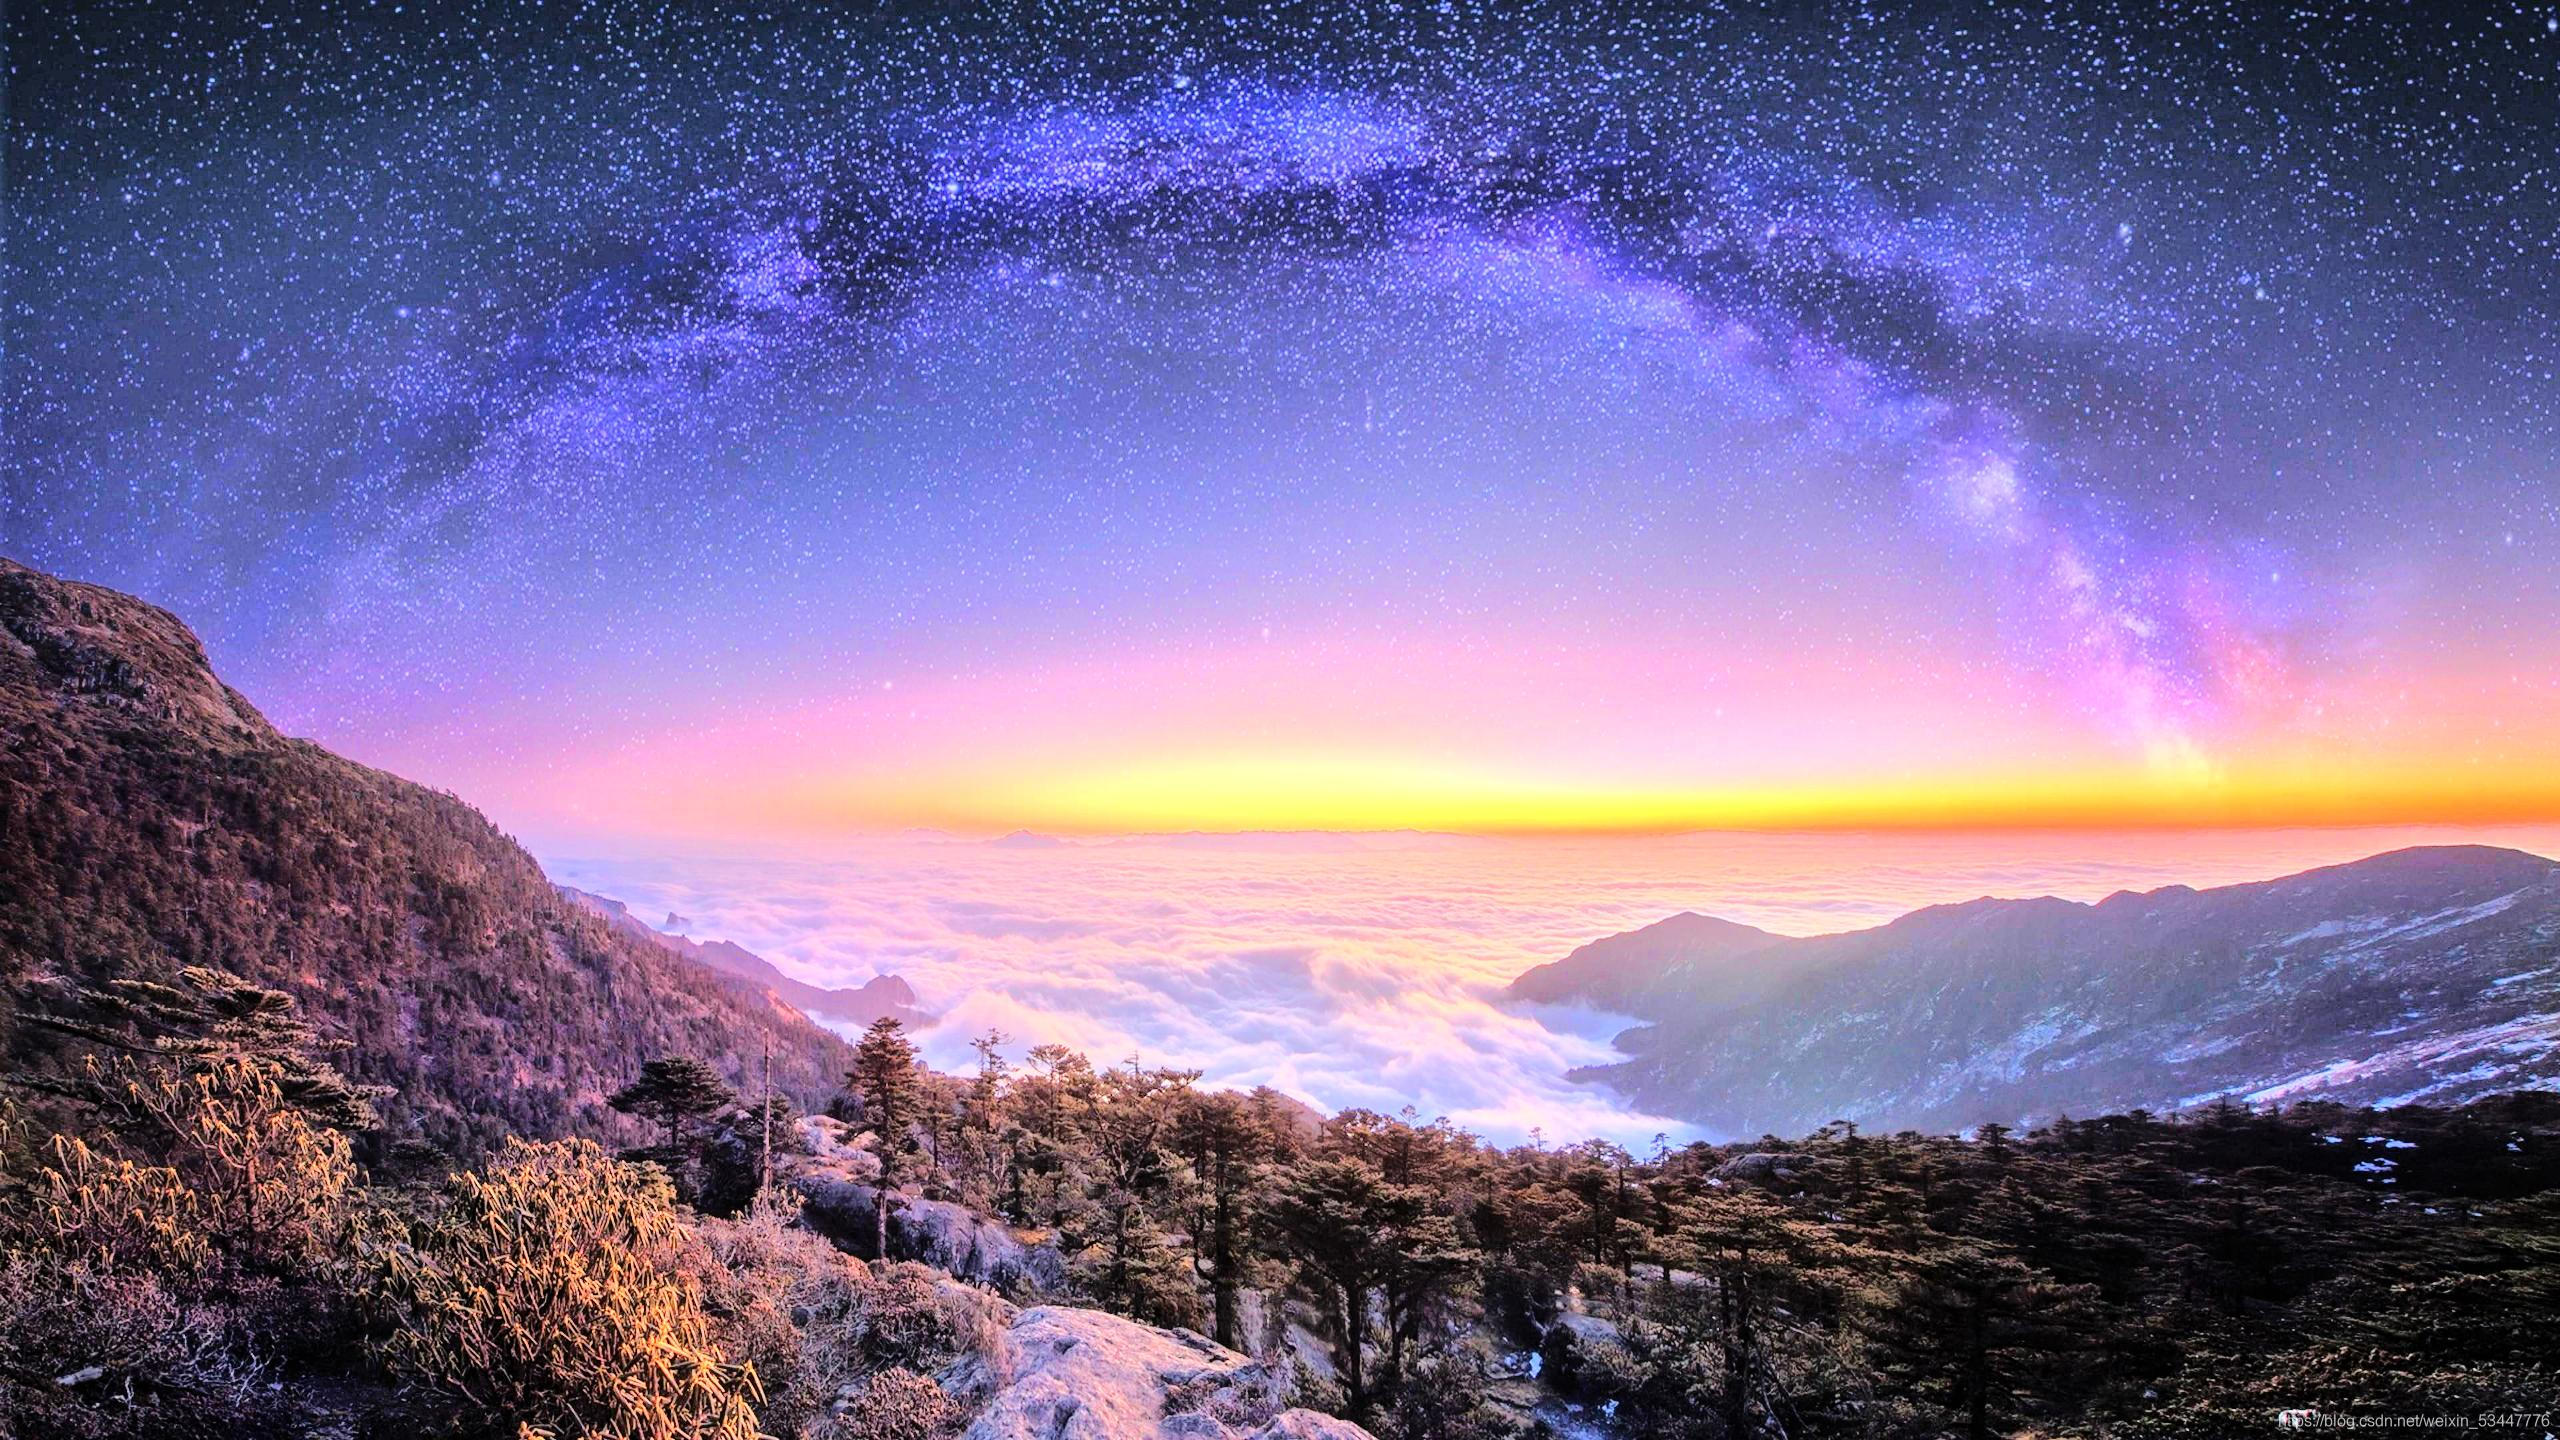
\includegraphics[width=0.5\linewidth]{ceshi.jpg}
  % 图片标题
  \captionof{figure}{图像模糊之前如下:}
  \label{fig:example}
\end{minipage}

\noindent
\begin{minipage}{\linewidth}
 \centering
  % 插入图片
  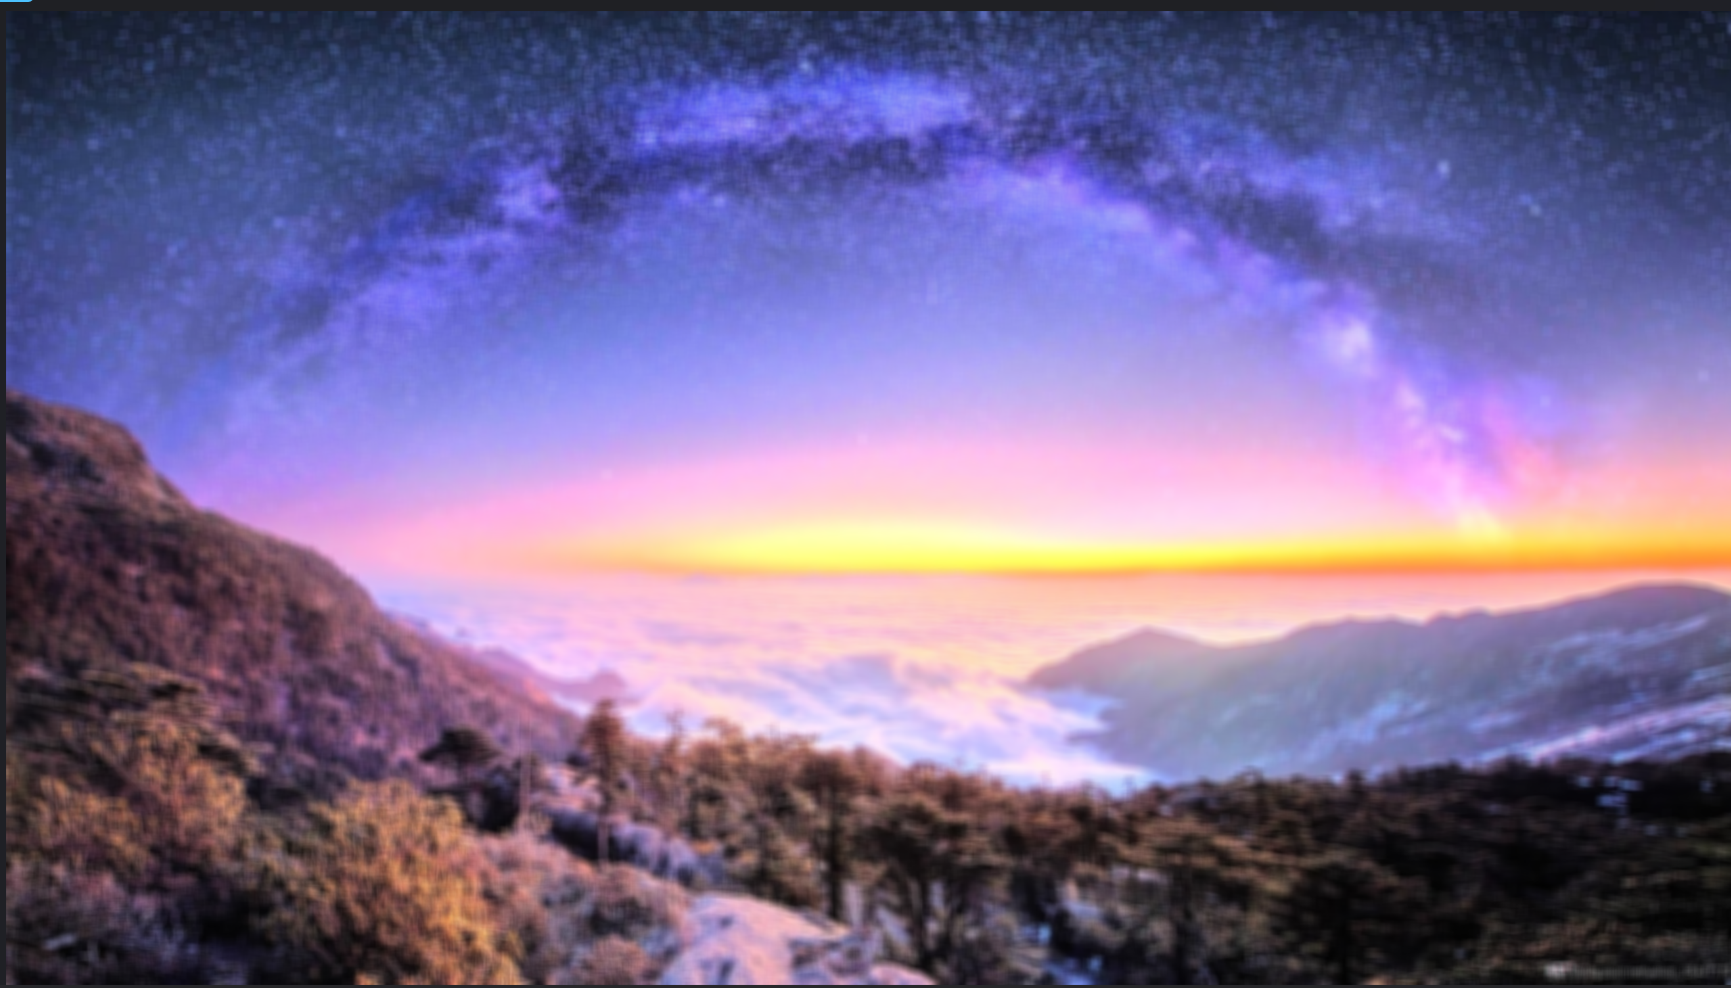
\includegraphics[width=0.5\linewidth]{mohu.png}
  % 图片标题
  \captionof{figure}{图像模糊之后如下:}
  \label{fig:example}
\end{minipage}

4.图像缩放
\begin{verbatim}
    import matplotlib.pyplot as plt
    # 读取图像
    image = plt.imread('ceshi.jpg')
    # 设置缩放比例
    scale_percent = 50  
    width = int(image.shape[1] * scale_percent / 100)
    height = int(image.shape[0] * scale_percent / 100)
    # 创建一个缩放后的图像
    resized_image = image[0:height, 0:width]
    # 显示缩放后的图像
    plt.imshow(resized_image)
    plt.axis('off')  # 不显示坐标轴
    plt.show()
  
\end{verbatim}


\noindent
\begin{minipage}{\linewidth}
 \centering
  % 插入图片
  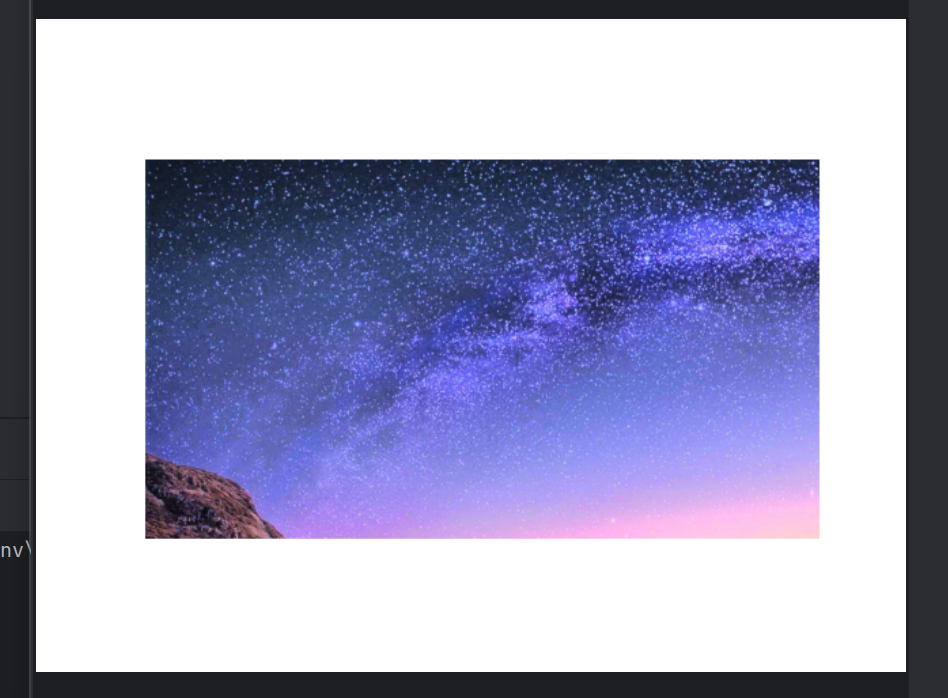
\includegraphics[width=0.5\linewidth]{suofang.png}
  % 图片标题
  \captionof{figure}{缩放后的图片}
  \label{fig:example}
\end{minipage}

5.缩略图绘制
\begin{verbatim}
    from PIL import Image
    # 读取原始图像
    original_image = Image.open('ceshi.jpg')  # 替换为您的图像路径
    # 设置缩略图的比例因子
    thumbnail_ratio = 0.25  # 缩略图尺寸是原始尺寸的25%
    # 创建缩略图
    thumbnail = original_image.resize((int(original_image.width * thumbnail_ratio), int(original_image.height * thumbnail_ratio)), Image.BICUBIC)
    # 显示原始图像和缩略图
    original_image.show()
    thumbnail.show()
\end{verbatim}


\noindent
\begin{minipage}{\linewidth}
 \centering
  % 插入图片
  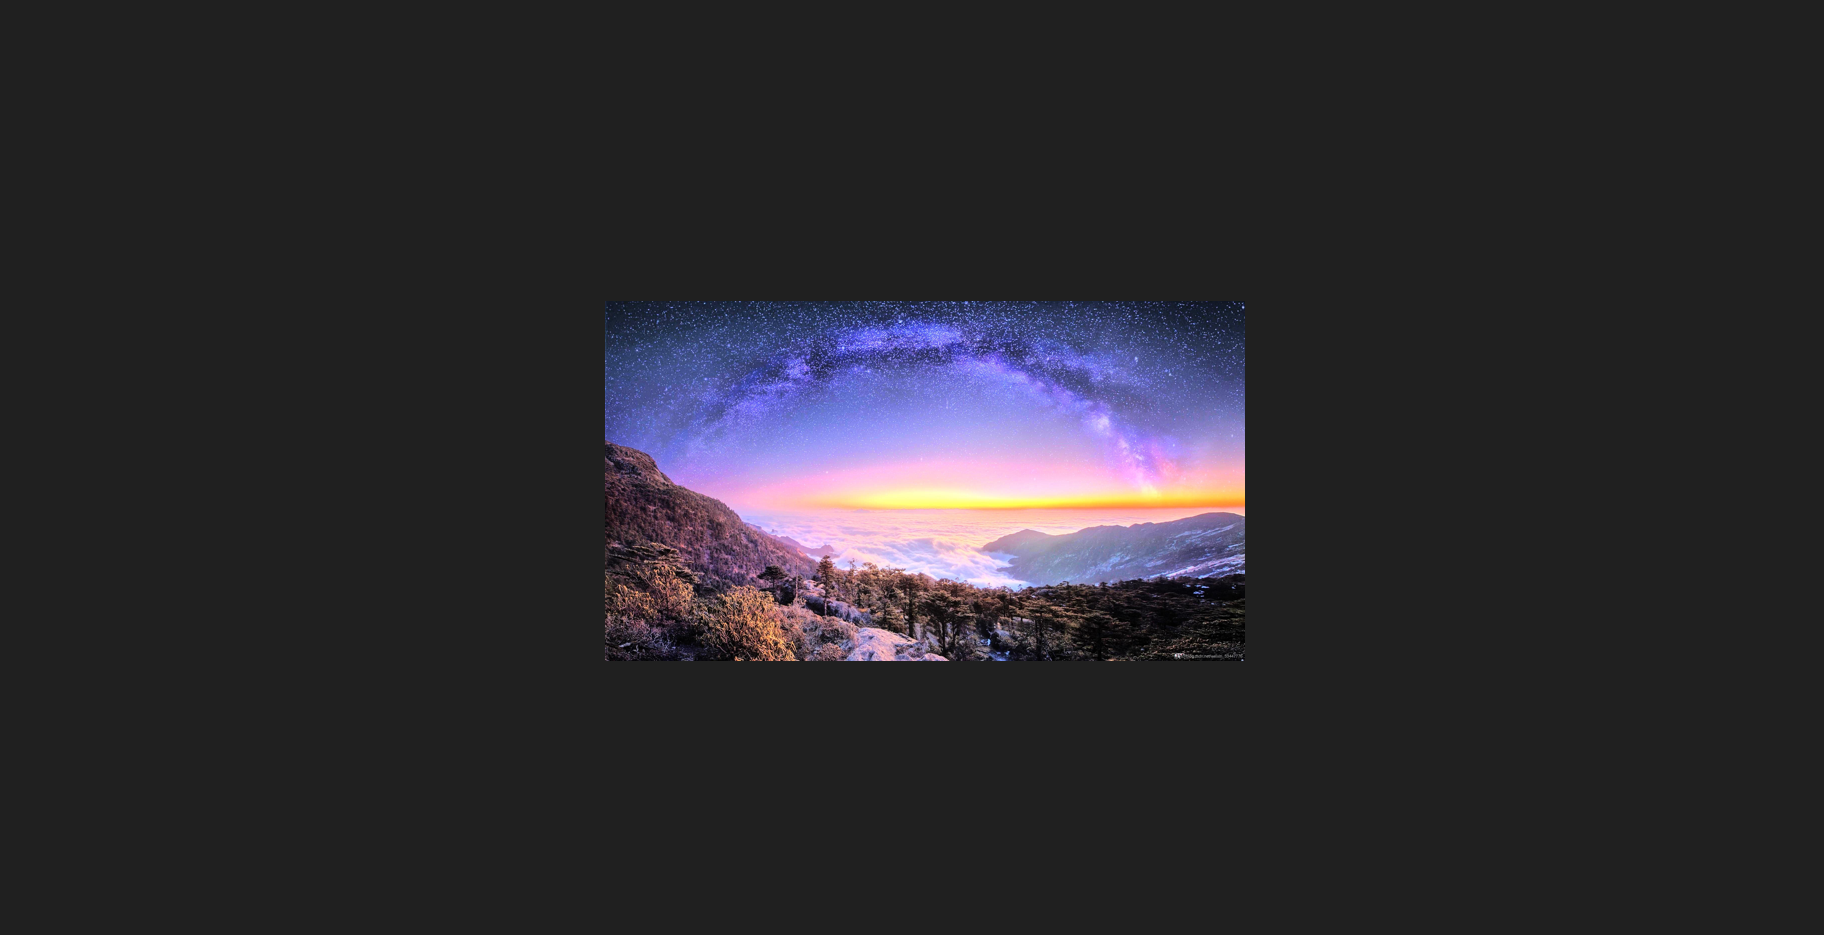
\includegraphics[width=0.5\linewidth]{suolue.png}
  % 图片标题
  \captionof{figure}{缩略图绘制}
  \label{fig:example}
\end{minipage}



\section{解题感悟}
Python是一种简便快捷的语言,非常容易入门。

Python的可视化能够将抽象的数据转化为直观的图像,这让信息变得更加易于理解。

通过命令行能够高效地与计算机系统互动,方便快捷地完成工作。

github路径
您可以在此查看项目的源代码: 

\url{https://github.com/L-c-hang/homework3}

\end{document}
